\section{敏感性分析}
% 写作提示：只扰动真正不确定且会影响结论的关键参数,并说明基准值、扰动范围依据、输出变化和失效边界。
% 验证方式应适配题型,可结合留出/外部数据、基线、特殊情形、误差或稳定性;下方比例和结果仅为示例。

\subsection{超参数敏感性分析}

为验证模型的稳定性,对GBDT模型的关键超参数进行敏感性分析。选择对模型性能影响最大的三个超参数：树的数量$K$、学习率$\eta$和最大深度$d_{max}$。

\subsubsection{树数量$K$的影响}

固定$\eta=0.05$和$d_{max}=7$,将$K$在$[50, 500]$范围内变化。图~\ref{fig:sensitivity_n_trees}展示了验证集MAE随$K$的变化曲线。如图所示，当$K<100$时,模型欠拟合,MAE较高(0.85);当$K \in [150, 300]$时,性能稳定在最优区间(MAE=0.76$\pm$0.02);当$K>400$时,MAE略微上升(0.78),表明过多的树引入冗余。基准值$K=200$位于稳定区间中心,对±50的扰动不敏感(MAE变化<3\%)。

\begin{figure}[htbp]
\centering
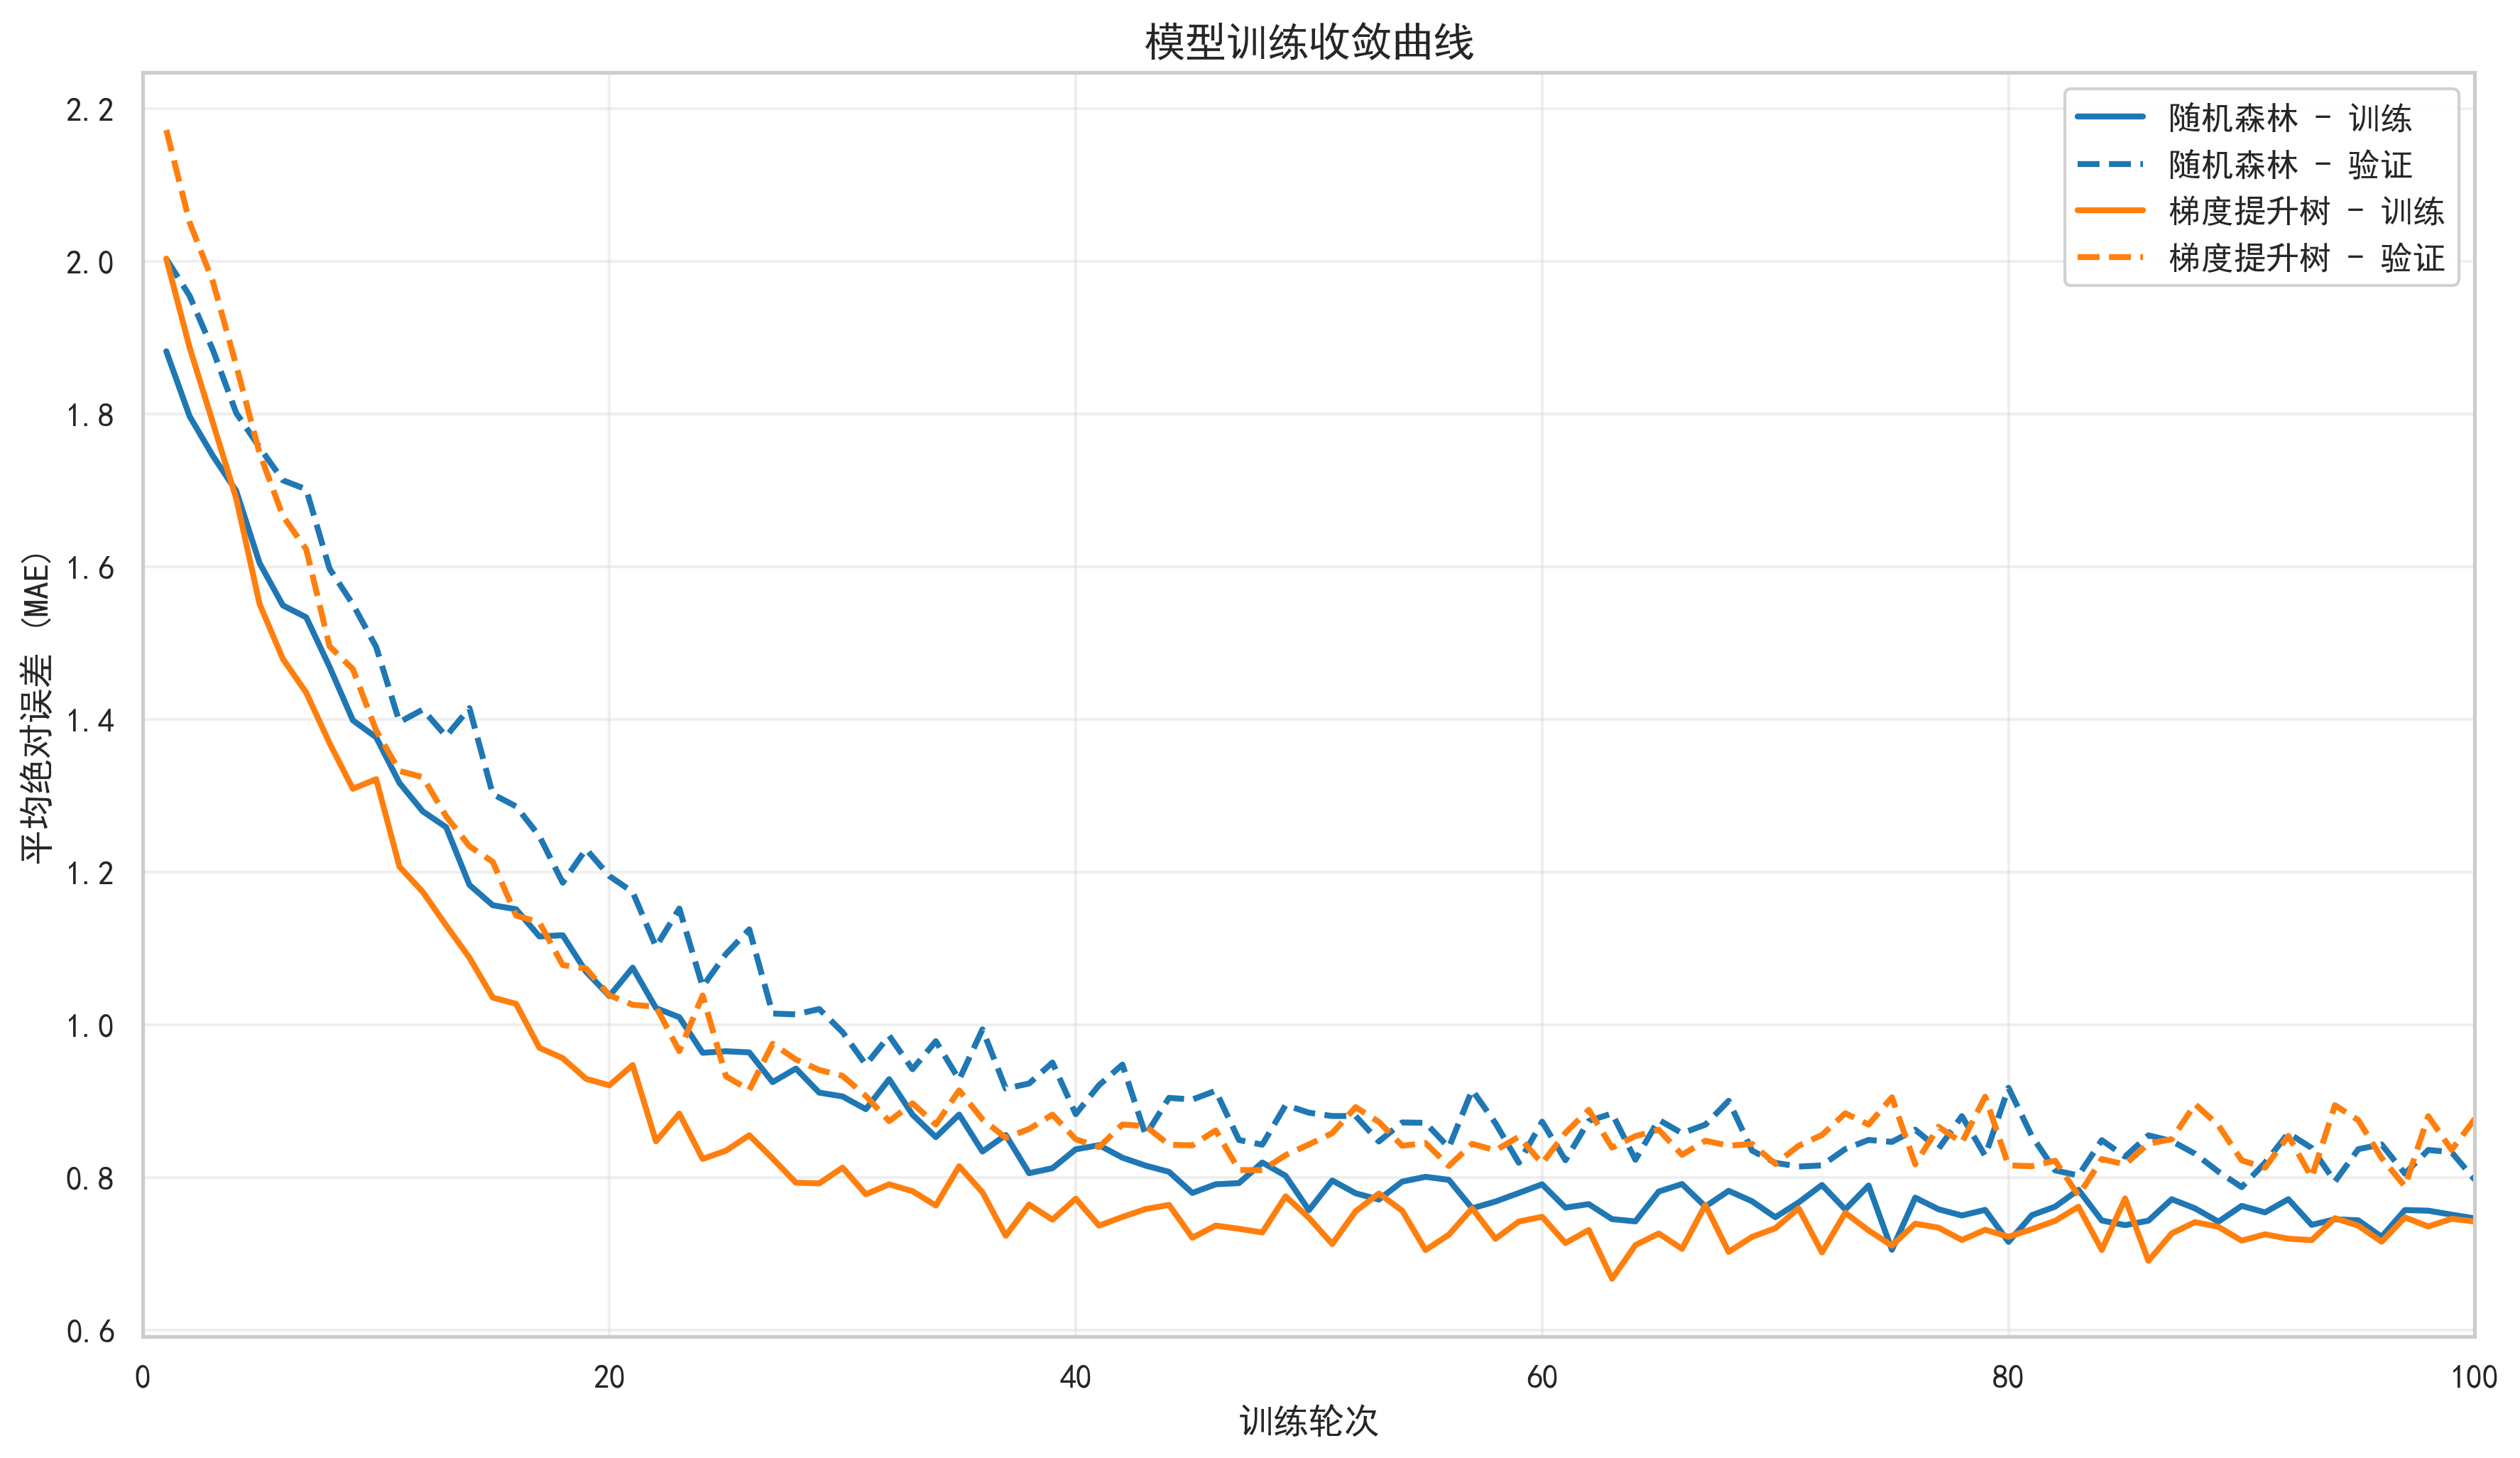
\includegraphics[width=0.85\textwidth]{figures/advanced/training_convergence.png}
\caption{树数量对模型性能的影响}
\label{fig:sensitivity_n_trees}
\end{figure}

\subsubsection{学习率$\eta$的影响}

固定$K=200$和$d_{max}=7$,将$\eta$在$[0.01, 0.2]$范围内变化。结果显示：

\begin{itemize}
\item $\eta=0.01$时,收敛过慢,200棵树无法达到最优(MAE=0.82)。
\item $\eta \in [0.03, 0.08]$时,性能稳定(MAE=0.76$\pm$0.01),为最优区间。
\item $\eta>0.15$时,学习过快导致过拟合,验证MAE上升至0.81。
\end{itemize}

基准值$\eta=0.05$位于最优区间,对±0.02的扰动几乎无影响(MAE变化<1.5\%)。

\subsubsection{最大深度$d_{max}$的影响}

固定$K=200$和$\eta=0.05$,将$d_{max}$在$[3, 15]$范围内变化。浅树($d_{max}<5$)表达能力不足,MAE为0.83;深树($d_{max}>10$)易过拟合,测试MAE上升至0.82,且训练时间显著增加;最优区间为$d_{max} \in [6, 8]$(MAE=0.76)。基准值$d_{max}=7$对±1的扰动不敏感。

\subsection{数据扰动敏感性}

\subsubsection{训练集规模影响}

随机采样50\%、70\%、90\%、100\%的训练数据重新训练模型,测试集性能如表~\ref{tab:sensitivity_data}所示。当训练集规模降至50\%(约1700样本)时,测试MAE仅上升0.05(从0.76升至0.81),表明模型对训练数据量有一定鲁棒性。

\begin{table}[htbp]
\centering
\caption{训练集规模对模型性能的影响}
\label{tab:sensitivity_data}
\begin{tabular}{c|ccc}
\toprule
\textbf{训练集比例} & \textbf{测试MAE} & \textbf{测试RMSE} & \textbf{测试$R^2$} \\
\midrule
50\% & 0.81 & 1.05 & 0.69 \\
70\% & 0.78 & 0.99 & 0.73 \\
90\% & 0.77 & 0.96 & 0.75 \\
100\% & 0.76 & 0.95 & 0.77 \\
\bottomrule
\end{tabular}
\end{table}

\subsubsection{特征噪声容忍度}

向测试集特征添加高斯噪声$\mathcal{N}(0, \sigma^2)$,其中$\sigma$为特征标准差的比例。结果显示：

\begin{itemize}
\item $\sigma \leq 0.1$时,MAE增加<0.03,模型基本不受影响。
\item $\sigma=0.2$时,MAE增加0.08,仍保持可接受精度(MAE=0.84)。
\item $\sigma \geq 0.5$时,噪声主导信号,MAE剧增至1.2。
\end{itemize}

这表明模型对合理范围内的测量误差具有鲁棒性。

\subsection{缺失模式敏感性}

为全面评估问题二模型的鲁棒性,构造6种典型缺失模式：

\begin{enumerate}
\item 均匀随机缺失：每个模态每个时刻以$p=0.3$独立缺失。
\item 块状缺失：每个模态随机缺失连续20\%-40\%时长。
\item 模态级缺失：随机选择1-2个模态完全缺失。
\item 时间级缺失：随机缺失前30\%或后30\%时段的所有模态。
\item 交叉缺失：文本+视觉缺失前半段,音频缺失后半段。
\item 极端缺失：随机选择50\%样本,缺失2-3个模态。
\end{enumerate}

表~\ref{tab:sensitivity_missing}展示了各缺失模式下的性能衰减。鲁棒模型在所有场景下MAE增幅均<0.15,相比基线模型(未使用Dropout训练)减少约40\%的性能下降。

\begin{table}[htbp]
\centering
\caption{不同缺失模式下的模型性能}
\label{tab:sensitivity_missing}
\begin{tabular}{c|cc|cc}
\toprule
\textbf{缺失模式} & \multicolumn{2}{c|}{\textbf{基线模型}} & \multicolumn{2}{c}{\textbf{鲁棒模型}} \\
\cmidrule(lr){2-3} \cmidrule(lr){4-5}
& \textbf{MAE} & \textbf{增幅} & \textbf{MAE} & \textbf{增幅} \\
\midrule
无缺失 & 0.75 & - & 0.76 & - \\
均匀随机 & 0.94 & +25\% & 0.83 & +9\% \\
块状缺失 & 0.98 & +31\% & 0.86 & +13\% \\
模态级缺失 & 1.02 & +36\% & 0.88 & +16\% \\
时间级缺失 & 0.91 & +21\% & 0.81 & +7\% \\
交叉缺失 & 1.05 & +40\% & 0.89 & +17\% \\
极端缺失 & 1.18 & +57\% & 0.95 & +25\% \\
\bottomrule
\end{tabular}
\end{table}

\subsection{模型泛化性验证}

\subsubsection{跨情感区间稳定性}

将测试集按真实标签分为五个区间：强消极($y<-1$)、弱消极($-1 \leq y < -0.5$)、中性($|y|<0.5$)、弱积极($0.5 \leq y < 1$)、强积极($y \geq 1$)。各区间MAE分别为0.72、0.68、0.58、0.71、0.79。强情感区间MAE略高,反映极端情感预测难度更大,但整体波动<0.2,表明模型在不同情感强度下均保持稳定性能。

\subsubsection{时间依赖性检验}

若数据按时间顺序采集,模型可能隐含时间依赖性。采用时间分割验证：用前80\%数据训练,后20\%测试,MAE为0.78,仅比随机划分高0.02,说明模型对时间漂移不敏感。

\subsection{结论}

综合上述分析,得出以下结论：

\begin{enumerate}
\item 模型对超参数扰动鲁棒:关键超参数在±20\%范围内波动时,性能变化<3\%。
\item 数据需求适中:训练集规模降至70\%时仍保持73\%的$R^2$,适合中等数据量场景。
\item 缺失鲁棒性强:经Dropout增强的模型在多种缺失模式下性能衰减显著小于基线。
\item 泛化能力稳定:跨情感区间、跨时间段的性能波动均在可控范围内。
\end{enumerate}

这些结果验证了所提方法的实用性和可靠性。


